\footnotesize
\makebox[\textwidth][c]{\begin{minipage}{400pt}
\textbf{Basic idea:} express the Q, K, V as functions of a lower-dim, `latent' activation
\begin{center}
\includegraphics[page=45,trim=297 211 297 95,clip,width=\linewidth,height=48pt,keepaspectratio]{figure/cs336-l4.pdf}\hspace{14pt}\includegraphics[page=45,trim=439 206 66 100,clip,width=\linewidth,height=48pt,keepaspectratio]{figure/cs336-l4.pdf}
\end{center}
\textbf{Benefits:} when KV-caching, we only need to store $c_t^{KV}$, which can be much smaller.
$W^{UK}$ can be merged into the Q projection\\
\mbox{}\hfill(they also compress queries, for memory savings during training)\quad\raisebox{-0.4\height}{\includegraphics[page=45,trim=561 110 72 239,clip,width=\linewidth,height=20pt,keepaspectratio]{figure/cs336-l4.pdf}}

\textbf{Complexity:} rope conflicts with MLA-style caching.\\[2pt]
\hspace*{1em}Without RoPE -- $\langle Q, K \rangle = \langle hW^Q, W^{UK} c_t^{KV} \rangle = \langle h\,\textcolor{red}{W^Q W^{UK}}, c_t^{KV} \rangle$\\[2pt]
\hspace*{1em}With RoPE -- $\langle QR_q, R_k K \rangle = \langle hW^Q R_q, R_k W^{UK} c_t^{KV} \rangle = \langle h\,\textcolor{red}{W^Q R_q R_k W^{UK}}, c_t^{KV} \rangle$\par\smallskip
{\centering\color{gray} The solution -- Have a few non-latent key dimensions that can be rotated\par}
\end{minipage}}
